\section{Meta-object system}
Meta-object system forms substantial part of Qt functionality, providing majority of Qt classes with ability to asynchronously report its state when something happens. Furthermore, you can equip even your cusom classes with extra textual information, fetch names of your objects\index{object} at run time or make your classes use of the custom \textit{property system}\index{property system} that provides faster and syntactically unified access to your class member data.

\begin{fdocextra}
The word \enquote{meta} (which is originally Greek preposition, in Greek written as \enquote{\textmu \textepsilon \texttau \textalpha} was for the first time used by \textit{Aristotle}, the great Greek philospher. Aristotle wrote plenty of writings, covering poetry, music or politics. His creations needed to be sorted later so that they could be interpreted correctly. Writings got sorted and scholars realized that there is one book with no name. It was placed \textit{after} Aristotle's great work \textit{Physics}. That's why that mysterious paper was named \textit{Metaphysics}, literally \enquote{the paper after Physics.}
\end{fdocextra}

\subsection{What is meta-object?}
Generally, meta-object is an entity that extends another object, providing us certain kind of information \textit{beyond} that particular object or set of objects. Meta-objects lie beyond actual objects, forming (kind of \enquote{higher}) abstraction layer of any Qt application. We can name this layer \textit{meta-echelon}\index{meta-echelon}.

Each class instance exposes its private data through \textit{methods} to its users -- other classes. Publicly available class members (methods or \textit{properties}\footnote{Property can be understood as private data member plus accessing getter/setter functions.}) form class interface, the only way to control class data and class behavior. This data is the only classical way to \enquote{see} the object from the view of its purpose but it says completely nothing about object inner structure and representation,\eg it doesn't expose type of on object (in run time) or count of its methods. Classic class methods do not provide us with \textit{meta-information}\index{meta-information}. Meta-objects do that.

\subsection{Reflection}
Ability to obtain and perhaps modify meta-information of any object is an action called \textit{introspection}\index{introspection} (or \textit{reflection})\index{reflection}. We can distinguish two kinds of reflection:
\begin{description}
\item[RUN TIME REFLECTION] \hfill \\
This is the superior way of reflection. Introspection of meta-information of certaing object is possible at runtime but with one important addition. Compiler supporting run time reflection has absolutely no need to know the basis for meta-information construction at compile time. It does not need to add any extra data to the output code to allow reflection. Reflection is natural part of the language. This kind of reflection is supported primarily by languages that profit from using virtual machine\index{virtual machine} and special output executable file structure. Both Java and .NET-based languages (\eg \csharp or Visual Basic) provide this.
\item[COMPILE TIME REFLECTION] \hfill \\
Compiler of compile time reflection supported language has to do extra work to make reflection available. It usually produces extra code that grabs all (or most of) meta-information at compile time by going through the source code and extracting property names, method names, class names and other needed information. Extracted information is then formed into certain aggregations that are available as meta-objects at run time.

This approach makes the compilation little slower because an extra tool has to be executed to do the job. This concerns Qt. Qt uses meta-object compiler\index{meta-object compiler}\index{moc} to produce meta-objects.
\end{description}

\subsection{Qt meta-object system}
Qt uses compilation-based reflection due to \cpp language limitations. Each object created within Qt meta-object system is automatically equipped with shadow meta-object. This meta-object allows you to do amazing things with that particular object. You can obtain its class name, check if this object's class inherits another class, get name of the supperclass or names of its methods. You can even call methods by their names stored in a string (\autoref{listing:invoke})! Complete example can be found in\fdocinlinecode{text}{!}{sources/laboratory/08-invoke} directory.

\begin{fdoccode}{cpp}{listing:invoke}{String-based method invokation in Qt meta-object system}
#include <QDebug>

#include <iostream>

#include "myapplication.h"


int main(int argc, char *argv[]){
    MyApplication a(argc, argv);
    
    std::string input;
    qDebug("Type name of method to be executed: ");
    std::cin >> input;
    QMetaObject::invokeMethod(&a, input.c_str());

    return a.exec();
}
\end{fdoccode}

\subsection{Enabling meta-object features for custom classes}
Not all classes in a Qt-based application take part in the meta-object system. You need to to several steps to make sure that objects of your class will acoompanied with coresponding meta-objects:

\begin{enumerate}
\item Your class needs to inherit\fdocinlinecode{cpp}{!}{QObject}. Public inheritance is recommended.\fdocinlinecode{cpp}{!}{QObject} class is fantastic base stone for any custom classes in Qt application. You will learn about it in the next chapter.
\item Your class needs to contain\fdocinlinecode{cpp}{!}{Q_OBJECT} macro in its private section, best way is right under class name. This macro adds several methods to your class, one of them is all important\fdocinlinecode{cpp}{!}{QMetaObject *metaObject() const}. Moreover, dynamic translation system is enabled by this macro too. You will learn about translating Qt applications later.
\end{enumerate}

\subsection{QObject class -- the cradle of meta-objects}
\fdocinlinecode{cpp}{!}{QObject} class is the very base class for each meta-object-system-enabled class and provides many marvellous features. It is good to use\fdocinlinecode{cpp}{!}{QObject} as the base class even for your custom classes within any Qt application because there is one particularly amazing feature -- the automatic memory management provided by \nameref{section:model}.

\subsubsection{Qt object model}\label{section:model}
There are some rules that apply to the way\fdocinlinecode{cpp}{!}{QObject} should be inherited. Copy constructor and assignment operator mustn't be implemented in inheriting class. Reasons are very simple:
\begin{enumerate}
\item Each and every\fdocinlinecode{cpp}{!}{QObject} instance stores pointer to its parent\fdocinlinecode{cpp}{!}{QObject} instance. This results in instance tree hierarchy (\autoref{figure:modeltree}). Should copy of\fdocinlinecode{cpp}{!}{QObject} instance point to the same parent?

\item Each\fdocinlinecode{cpp}{!}{QObject} instance has certain properties and those can be unique. Example of such a property could be instance name (can be set by\fdocinlinecode{cpp}{!}{void	QObject::setObjectName(const QString & name)} function) which \textbf{must be} unique for each\fdocinlinecode{cpp}{!}{QObject} instance. You could assign the same name to the new copy of the instance but that results in two instances with the same name (\autoref{figure:samenames}) and that's the problem because:
\begin{enumerate}
\item You may want to search for one particular object by name which is possible in Qt. Two objects with the same name make search ambiguous.
\item You don't know where to place new copy in the tree hierarchy. It could be positioned as the sibling of the original object. Problem becomes clear when you try to free original \enquote{George} instance from memory. All its children are removed too, in other words, whole subtree with \enquote{George} as the root gets cleared from application memory but another (cloned) \enquote{George} remains untouched. Is this desired behavior? In some situations it could be but mostly it's not.
\end{enumerate}
\end{enumerate}

\begin{figure}[ht]
\centering
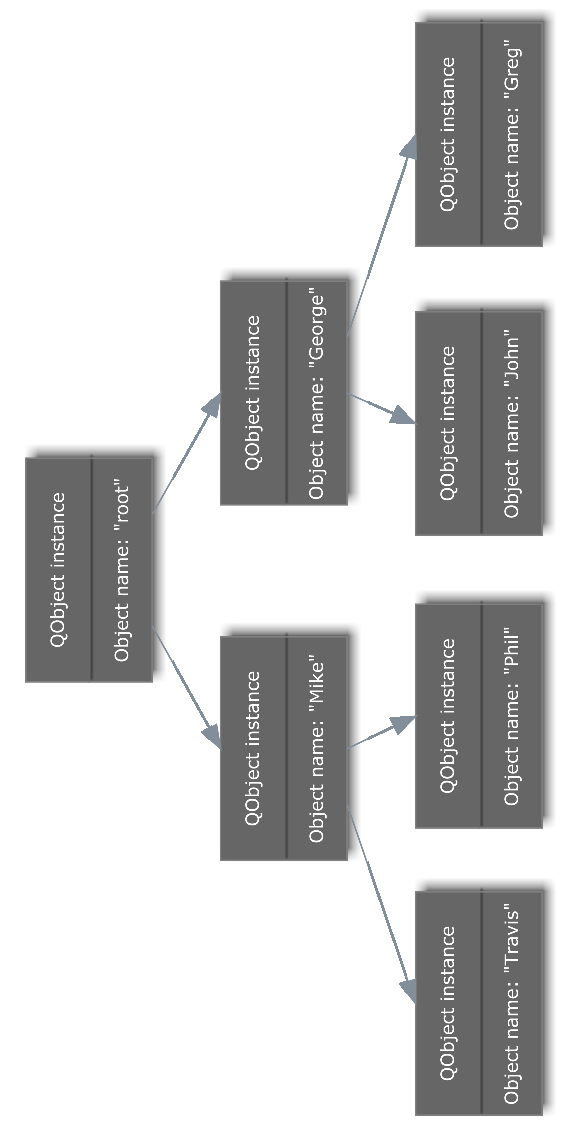
\includegraphics[angle=-90,width=13cm]{graphics/laboratory/12-modeltree.pdf}
\caption{QObject instances tree hierarchy}\label{figure:modeltree}
\end{figure}

\begin{figure}[ht]
\centering
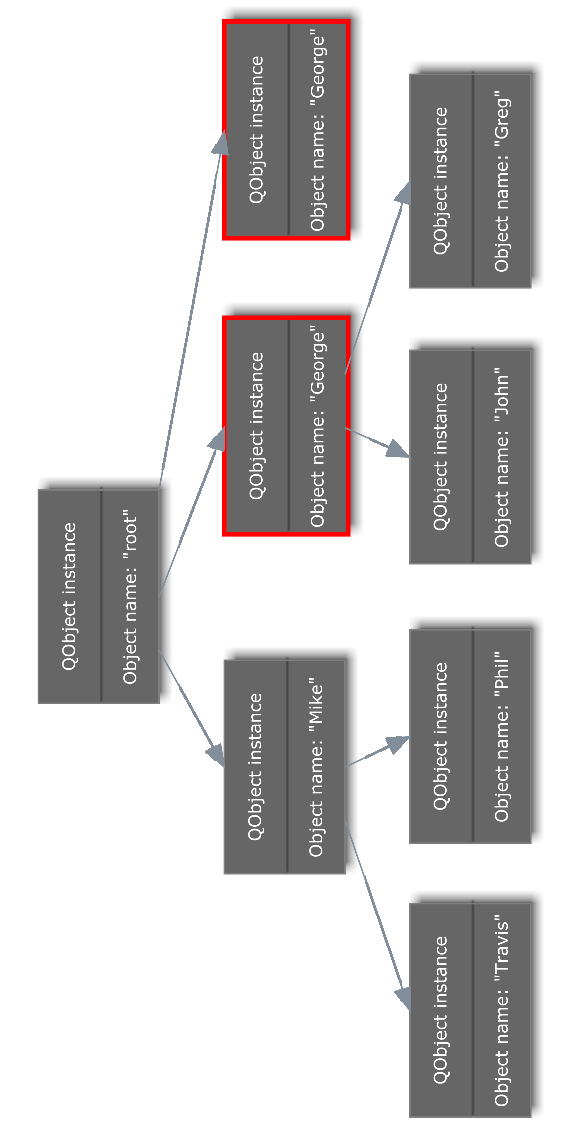
\includegraphics[angle=-90,width=13cm]{graphics/laboratory/13-samenames.pdf}
\caption{Broken QObject instances tree hierarchy}\label{figure:samenames}
\end{figure}

\subsubsection{Subclassing QObject}
% popsat jak dědit QObject

\subsubsection{Events}
% metoda QObject::startTimer...událost dále customEvent

\subsubsection{Signal--slot mechanism}

\subsubsection{QObject instance life cycle}
% Q_OBJECT, QObject, object model, metaobject compiler, property system (a možná events)